\documentclass[12pt,a4paper]{article}
\usepackage{graphicx}

\author{Akash Kishore}
\title{\textbf{My First {\LaTeX} Document}}
\date{22 April 2020}

\begin{document}
	\maketitle
	\begin{abstract}
	I want to learn how to use {\LaTeX} for idk what reason, it seem's \textsl{cool} is all I know. 
	\end{abstract}
	\tableofcontents
	\section{A List}
	Here is a itemised list :
	\begin{enumerate}
		\item Hello this is \emph{$E=mc^2$}
		\item Hello this is \textbf{\underline{Item 2}}
		\item Look at this $ T^{i_1,i_2 \dots i_n}_{j_1,j_2 \dots j_n} = \int_{e^{-x}}^{e^{x}} \frac{\sin(\Delta x)*\cos(y)}{\tanh(xy)}dxdy$
		\item Say hello to tables $\rightarrow$
			\begin{tabular}{| c | c | c |}
			\hline
			Column 1 & Column 2 & Column 3 \\ [0.5ex]
			\hline
			1 & 2 & 33333333333333 \\
			\hline
			4 & 5123456789 & 6 \\
			\hline
			7 & 8 & 9 \\
			\hline
			\end{tabular}
	\end{enumerate}
	\begin{figure}
		\centering
		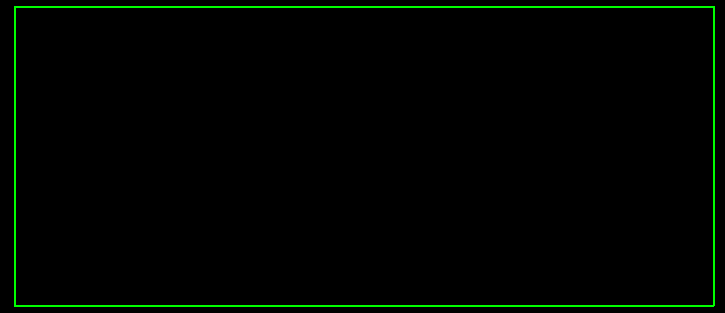
\includegraphics[width=0.5\textwidth]{greenbox}
		\caption{First Image}
		\label{fig:image1}
	\end{figure}
\end{document}